\documentclass[12pt, a4paper]{article}

% Pacotes essenciais:

% CONFIGURAÇÕES DE IDIOMA E CODIFICAÇÃO
\usepackage[utf8]{inputenc}
\usepackage[T1]{fontenc}
\usepackage[brazilian]{babel}

% FORMATAÇÃO E ESTRUTURA DO DOCUMENTO
\usepackage{geometry}
\usepackage{setspace}
\usepackage{float}
\usepackage{subcaption}

% MATEMÁTICA E EXPRESSÕES
\usepackage{amsmath}

% TABELAS
\usepackage{booktabs}
\usepackage{tabularx}
\usepackage{array}
\usepackage{longtable}

% FIGURAS E GRÁFICOS
\usepackage{graphicx}
\usepackage{pgfplots}
\pgfplotsset{compat=1.18}

% ALGORITMOS E PSEUDOCÓDIGO
\usepackage[ruled,vlined,linesnumbered]{algorithm2e}

% Tradução dos elementos do algoritmo
\SetAlgorithmName{Algoritmo}{algoritmo}{Lista de Algoritmos}
\SetKwInput{KwIn}{Entrada}
\SetKwInput{KwOut}{Saída}

% HIPERLINKS E REFERÊNCIAS
\usepackage{hyperref}


%comandos editaveis
\newcommand{\disciplina}{INSTRUMENTAÇÃO ELETRÔNICA}

\newcommand{\titulo}{Calibração Estática do Acelerômetro MPU-6050 e Medição de
Ângulo de Inclinação}

\newcommand{\aluno}{ Mateus Souza Santana - 200024841 }


% Configuração das margens
\geometry{a4paper, left=3cm, top=3cm, right=2cm, bottom=2cm}

% Configuração de cabeçalho e rodapé
\usepackage{fancyhdr}
\pagestyle{fancy}
\fancyhf{} % Limpa os cabeçalhos e rodapés atuais
\lhead{UnB} % Canto superior esquerdo
\rhead{\disciplina} % Canto superior direito
%\lfoot{Universidade de Brasília} % Canto inferior esquerdo
\rfoot{\thepage} % Canto inferior direito
\renewcommand{\headrulewidth}{0.4pt}
%\renewcommand{\footrulewidth}{0.4pt}

\begin{document}

% --- Título ---
\begin{center}
    {\Large \textbf{ \titulo }}\\[0.5cm]
    {\large \aluno}\\[0.2cm]
    {\normalsize \today}\\[1cm]
\end{center}

% --- Seções do Relatório ---
\section*{Resumo}

Este relatório descreve a calibração estática e a validação experimental de um inclinômetro embarcado baseado no acelerômetro triaxial MEMS MPU-6050 (GY-521) e bi microcontrolador ESP32 DevKit. A caracterização nas seis orientações ortogonais ($\pm 1 \text{ g}$ por eixo) revelou um offset elevado no eixo X (+1,322 g), motivando a adoção da escala $\pm 4 \text{ g}$ (8192 LSB/g) com  filtro passa-baixas digital (DLPF) de 5 Hz. Os ganhos estimados (0,98591; 0,98939; 1,01413) apresentaram desvio inferior a 1,5\% do valor unitário. O ângulo foi estimado via função atan2 no plano XZ e validado em plataforma impressa em 3D com transferidor entre 10° e 140°, antingindo alta precisão eletrônica ($\sigma$ médio de 0,129°;$R^2 = 0,9989$), RMSE de 7,228° e erro máximo de 10,862°, dominados por efeitos mecânicos do aparato. 

\vspace{0,5cm}

{\raggedright
\textbf{Palavras-chave:} Acelerômetro MEMS, calibração estática, ESP32, instrumentação eletrônica, medição de inclinação, MPU-6050.}

\vspace{0,5cm}

\section{Introdução}

A medição de inclinação angular é essencial em aplicações de robótica, monitoramento estrutural, estabilização de plataformas e controle industrial \cite{1.doebelin2004}. Acelerômetros microeletromecânicos (MEMS) de baixo custo
viabilizam essa medição em regime estático pela projeção do vetor gravidade sobre três eixos ortogonais \cite{2.pedley2013}. Contudo, imperfeições de fabricação, soldagem e estresse mecânico introduzem erros sistemáticos de deslocamento de zero (\textit{offser}) e sensibilidade (\textit{ganho}) que degradam os cálculos trigonométricos se não compensados por uma calibração estática criteriosa \cite{3.fisher2010}, \cite{4.ochoa2026}.

Neste trabalho, foi realizado a calibração e validação de um onclinômetro de um grau de liberdade com o MPU-6050 e o ESP32 DevKit \cite{4.ochoa2026}. OS objetivos rdprvcíficos são: 

\begin{enumerate}
    \item selecionar a escala e a filtragem digital adequadas;

    \item estimar ganho e offset nos três eixos pelo método das seis posições ($\pm 1$ \text{ g})

    \item calcular o ângulo de inclinação em tempo real com embasamento na literatura;

    \item a curva de erro frente a um transferidor acoplado a um mecanismo impresso em 3D.
\end{enumerate}
\section{Desenvolvimento}

% =====#=====#=====#===== %

\subsection{Hardware e Plataforma de Validação}
O sistema emprega um módulo GY-521 com sensor MPU-6050 (ADC de 16 bits por eixo) \cite{5.invensense2013spec} conectado a um ESP32 DevKit (Arduino IDE) via IC a 400 KHZ (endereço 0x68, GPIO 21/SDA e GPIO 22/SCL). Embora a escala de $\pm 2 \text{ g}$ (16384 LSB/g) maximize a resolução nominal, testes preliminares identificaram offset superior a +1,3 g no eixo \textbf{X}, o que causaria saturação em +1 g ($+2,3 \text{ g} > 2 \text{ g}$). Configurou-se, portanto, o registrador ACCEL\_Config (0x1C) para $\pm 4 \text{ g}$ (AFS\_SEL = 1; 8192 LSB/g, resolução melhor qye 0,01°/LSB), com filtro DLPF em 5 Hz (CONFIG = 0x06) e amostragem de 100 Hz (SMPLRT\_DIV = 0x09) \cite{6.invensense2013register}. 

A Figura~\ref{fig:estrutura} Apresenta a estrutura articulada impressa em 3D com dois níveis bolha ortogonais embutidos no bloco do GY-521 para auxiliar o nivelamento \cite{4.ochoa2026} e o transferido de 0° a 180° acoplado lateralmente para validação em um grau de liberdade.

\begin{figure}[h]
    \centering

    \begin{subfigure}{0.3\textwidth}
        \centering
        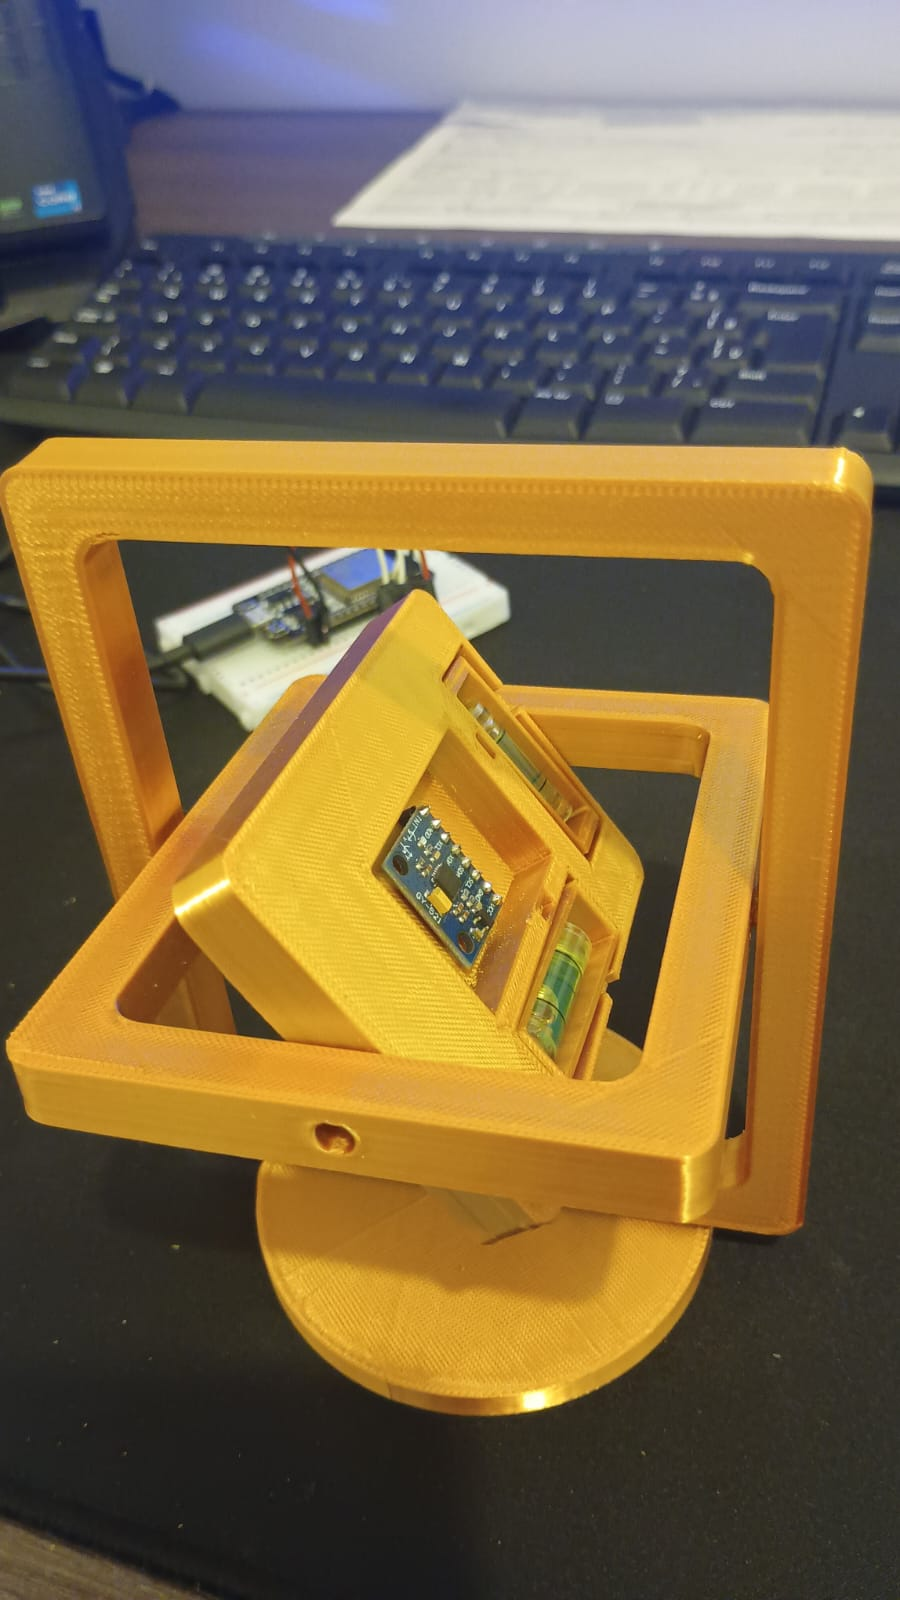
\includegraphics[width=\textwidth]{IMG/plataforma.jpeg}
        \caption{Suporte 3D com GY-521}
        \label{fig:imagem1}
    \end{subfigure}
    \hspace{0.5cm}
    \begin{subfigure}{0.3\textwidth}
        \centering
        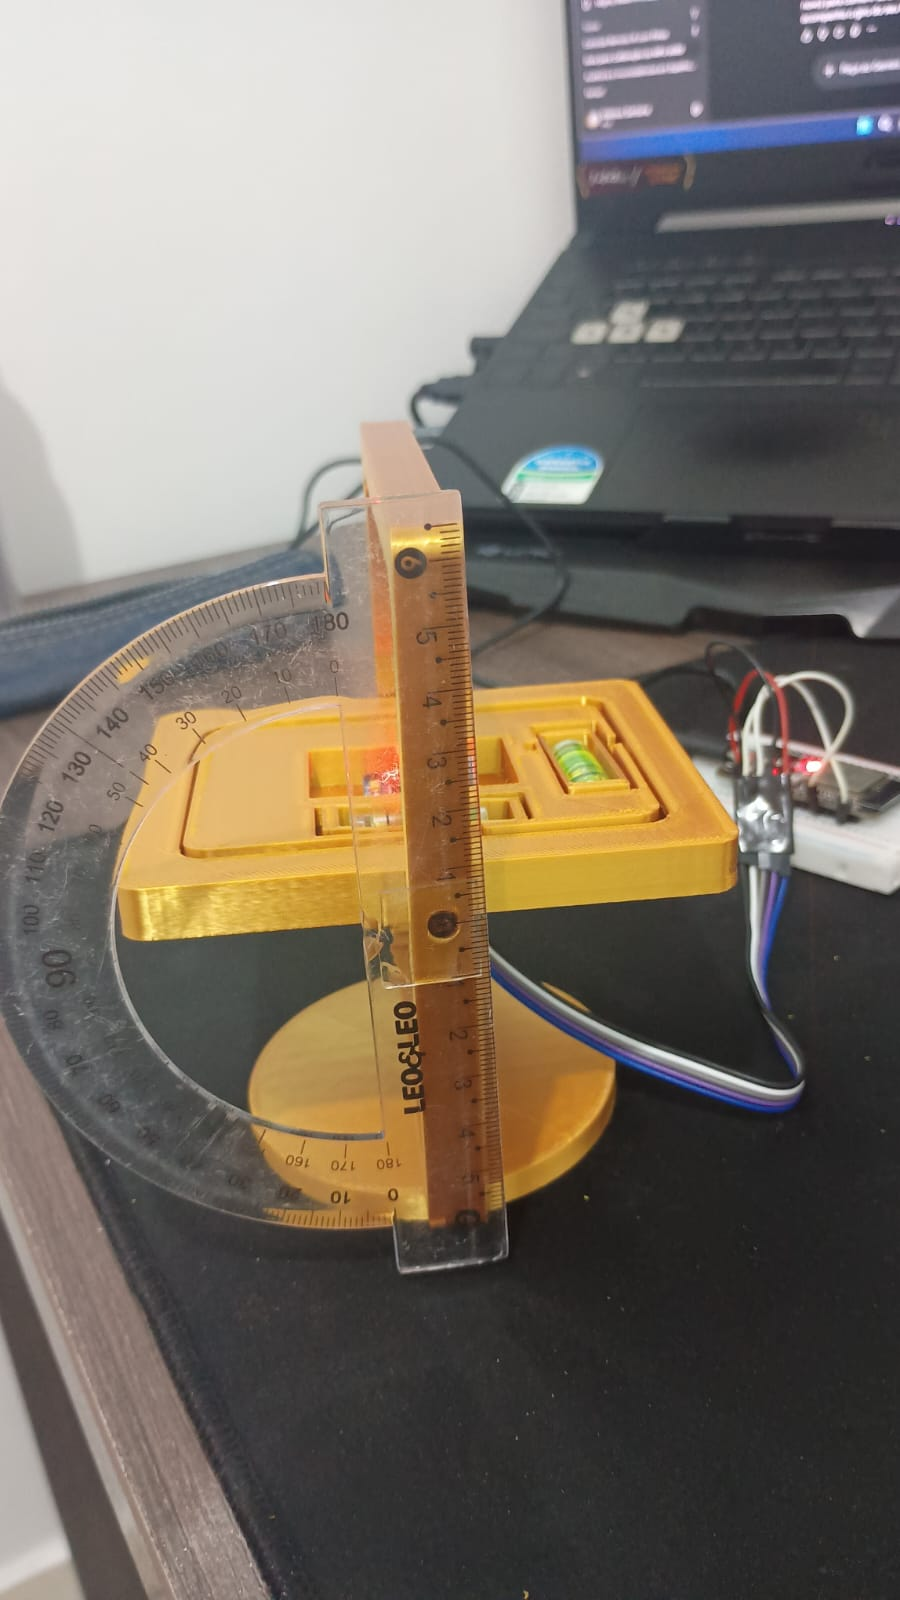
\includegraphics[width=\textwidth]{IMG/sistema.jpeg}
        \caption{Transferidor em 90°}
        \label{fig:imagem2}
    \end{subfigure}

    \vspace{0.2cm}

    \caption{Aparato experimental: (a) plataforma 3D com GY-521, níveis bolha e ESP32 ao fundo; (b) conjunto com transferidor (0° a 180°) na referência horizontal de 90°.}
    \label{fig:estrutura}
\end{figure}

% =====#=====#=====#===== %

\subsection{Calibração Estática do Acelerômetro}
Modelou-se a saída estática de cada eixo $i \in \{X, Y, Z\}$ em [$g$] por uma relação linear frente à aceleração de referencia $A_{ref}$ \cite{4.ochoa2026}

\begin{equation}
    A_{saída} = Ganho_i \times A_{ref} \times A_{offset,i}
    \label{eq:equacao_1}
\end{equation}

Alinhando cada eixo às seis orientações ortogonais ($\pm 1 \text{ g}$) sobre superfície nivelada e coletando N=200 amostras por posição (acima do mínimo de 100 exigidos \cite{4.ochoa2026}), obtiveram-se as médias $\bar{A}_{+1g,i} \text{ e } \bar{A}_{-1g,i}$. Resolvendo o sistema de \ref{eq:equacao_1} avaliada em $+1 \text{ g e } -1 \text{ g}$, determinam-se os parâmetros e a equação de compensação em tempo real:

\begin{equation}
    Ganho_i = \bar{A}_{+1g,i} - \bar{A}_{-1g,i}2 \text{, } \bar{A}_{offset,i} = \bar{A}_{+1g,i} + \bar{A}_{-1g,i}2 \text{, } \bar{A}_{cal,i} = A_+{saída,i} - A_{offset,i}Ganho_i
    \label{eq:equacao_2}
\end{equation}

A Tabela~\ref{tab:parametro_calibracao} resume os parâmetros estimados. Todos os ganhos ficaram a menos de 1,5\% da unidade, confirmando boa linearidade mesmo com o  offset acentuado em X ($+1,32212 \text{ g}$). 


\begin{table}[htbp]
    \centering
    \caption{Parâmetros de Calibração Estática do MPU-6050 (Escala $\pm4 \text{ g, }N = 200$ Amostras/Posição)}
    \label{tab:parametro_calibracao}
    
    \resizebox{\textwidth}{!}{%
    \begin{tabular}{c c c c c c c}
        \toprule
        \textbf{Eixo}                        & 
        \textbf{Média $\bar{A}_{+1g,i}$ [g]} & 
        \textbf{Média $\bar{A}_{-1g,i}$ [g]} & 
        \textbf{Ganho (adim.)}               & 
        \textbf{Desvio}                      & 
        \textbf{$A_{ofsset}$ [g]} \\
        \midrule
        
        \textbf{X} & $+2,30804$ & $+0,33621$ & $0,98591$ & $-1,41\%$ & $+1,32212$ \\
        \textbf{Y} & $+1,25741$ & $-0,72137$ & $0,98939$ & $-1,06\%$ & $+0,26802$ \\
        \textbf{Z} & $+0,85081$ & $-1,17746$ & $1,01413$ & $+1,41\%$ & $-0,16333$ \\
                
        \bottomrule
    \end{tabular}%
    }
    
    \vspace{0.2cm}
    
    \raggedright
    \footnotesize
    Fonte: Elaborado pelo autor (2026).
\end{table}

% =====#=====#=====#===== %

\subsection{Cálculo do Ângulo de Inclinação}
Conforme as notas de aplicação AN3461 (Freescale/NXP) \cite{2.pedley2013} e AN-1057 (Analog Devices) \cite{3.fisher2010}, funções de eixo único (arcsin ou arccos) perdem sensibilidade próximo aos extremos ($\pm90° \text{ ou  } 0°$), amplificando o ruído. Adotou-se, portanto, a função \textit{atan2} no plano XZ (toyação em torno de Y), que mantém sensibilidade constante, elimena ambiguidade de quadrante e independe da magnitude exta da gravidade \cite{2.pedley2013}, \cite{3.fisher2010}. como a horizontal ($atan2 = 0°$) coincide com $90°$ no transferido da Figura~\ref{fig:imagem2}, somou-se $90°$ para leitura direta ($0° \text{ a } 180°$), definindo-se também o erro de estimativa $e_K$ \cite{4.ochoa2026}:

\begin{equation}
    \theta_{med} = 90° + atan2(A_{cal,x},A_{cal,z}) \times 180°\pi \text{ ; } e_K = \theta_{med,K} - \theta_{ref,K}
    \label{eq:equacao_3}
\end{equation}

% =====#=====#=====#===== %

\subsection{Lógica Implementada e Repositório}
O firmware no ESP32 oferece menu serial com três rotinas: calibração guiada, validação com saída CSV (média e desvio padrão de 100 amostras) e monitoramento contínuo para demonstração (Algoritmo 1).


\begin{algorithm}[H]
\caption{Calibração, Compensação e Estimação Angular no ESP32}
\label{alg:calibracao_esp32}

\small
\ttfamily
\SetAlgoNoLine
\DontPrintSemicolon
\SetAlgoNoEnd

INÍCIO\;

\Indp
Iniciar Serial (115200 bps) e I2C (SDA=21, SCL=22, 400 kHz)\;

Configurar MPU-6050: Wake(0x6B=0x00), DLPF 5Hz(0x1A=0x06), 100Hz(0x19=0x09), $\pm$4g(0x1C=0x08)\;

SE modo == CALIBRAÇÃO ENTÃO\;

\Indp
PARA i EM \{X, Y, Z\} FAÇA\;

\Indp
Coletar médias $\bar{A}(+1g,i)$ e $\bar{A}(-1g,i)$ sobre 200 leituras brutas (/ 8192,0)\;

Ganho[i] $\leftarrow$ ($\bar{A}(+1g,i)$ - $\bar{A}(-1g,i)$) / 2 ; Offset[i] $\leftarrow$ ($\bar{A}(+1g,i)$ + $\bar{A}(-1g,i)$) / 2\;

\Indm
FIM PARA; Exibir tabela de parâmetros\;

\Indm
SENÃO (VALIDAÇÃO ou TEMPO\_REAL)\;

\Indp
ENQUANTO ativo FAÇA\;

\Indp
Ler aceleração bruta [g] e compensar: A_cal[i] $\leftarrow$ (A_bruta[i] - Offset[i]) / Ganho[i]\;

$\theta_{med}$ $\leftarrow$ 90,0 + atan2(A_cal[X], A_cal[Z]) * (180,0 / $\pi$)\;

SE VALIDAÇÃO: calcular média e $\sigma$ de 100 leituras, e $\leftarrow$ $\theta_{med}$ - $\theta_{ref}$, imprimir CSV\;

SENÃO: exibir A_cal[X,Y,Z], módulo |A| e $\theta_{med}$ continuamente no terminal\;

\Indm
FIM ENQUANTO\;

\Indm
FIM SE\;

\Indm
FIM

\end{algorithm}

{\raggedright
\textbf{Repositório:} Códigos do ESP32 e scripts de análise em: \href{https://github.com/mateus-ss/calibracao_MPU-6050}{calibracao\_MPU-6050}}
\section{Resultados e Discussão}

Na checagem estática pós-calibração ha horizontal ($90°$ na Figura~\ref{fig:imagem2}), oito leituras consecutivas apresentaram $A_{cal,z} \text{ entre } +0,998 \text{ g e } +1,012 \text{ e}$, componentes horizontais próximas de zero ($A_{cal,x} \in [-0,030; -0,019] \text{ g; } A_{cal,y} \in [-0,027; -0,013] \text{ g}$) e normal |A| entre $0,999 \text{ g}$ e $1,012 \text{ g}$ (média $1,005 \text{ g}$), confirmando a remoção do offset de +$1,322 \text{ g}$ em \textbf{X}. Em seguida Validou-se o sistema de 10° a 140° (Tabela~\ref{tab:validacao} e Figura~\ref{fig:grafico}{}), consolidando o ponto de 30° pela média das aquisições realizadas. 


\begin{table}[htbp]
    \centering
    \caption{Validação Angular com Transferidor (N = 100 Leituras por Ponto)}
    \label{tab:validacao}
    
    \resizebox{\textwidth}{!}{%
    \begin{tabular}{c c c c}
        \toprule
        \textbf{Referência $\theta_{ref} \text{ [°]}$}              & 
        \textbf{Estimado $\theta_{med} \text{ [°]}$}                & 
        \textbf{Erro $e = \theta_{med} - \theta_{ref} \text{ [°]}$} & 
        \textbf{Desvio Padrão $\sigma \text{ [°]}$}                 \\
        \midrule
        
        10,00  & $20,862$  & $+10,862$ & $0,123$ \\
        30,00* & $40,659$  & $+10,659$ & $0,164$ \\
        50,00  & $55,574$  & $+5,574$  & $0,172$ \\
        80,00  & $78,007$  & $-1,993$  & $0,119$ \\
        90,00  & $88,141$  & $-1,859$  & $0,096$ \\
        100,00 & $97,248$  & $-2,752$  & $0,165$ \\
        120,00 & $112,918$ & $-7,082$  & $0,091$ \\
        140,00 & $130,503$ & $-9,497$  & $0,071$ \\
                
        \bottomrule
    \end{tabular}%
    }
    
    \vspace{0.2cm}
    
    \raggedright
    \footnotesize
    Fonte: Elaborado pelo autor (2026).
\end{table}

{\raggedright
\textit{\textbf{*}Média de duas aquisições em 30,00° ($43,143°$ com $\sigma = 0,096°$ e $38,174°$ com $\sigma = 0,232°$)}}

\begin{figure}[H]
    \centering
    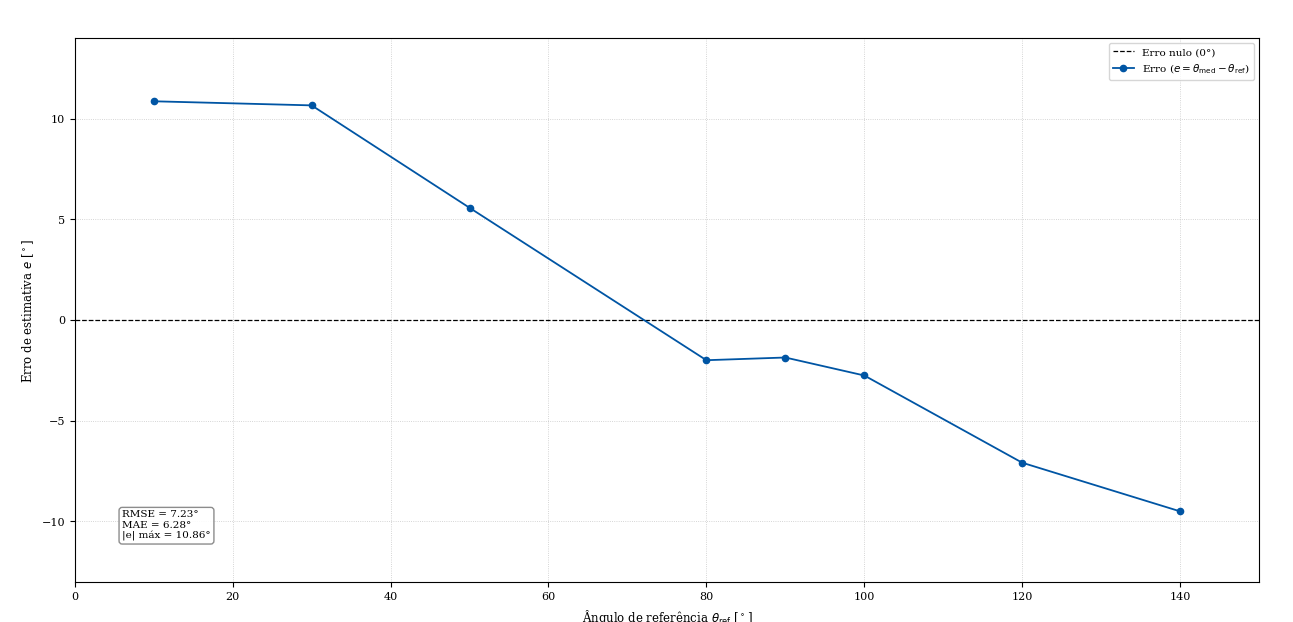
\includegraphics[width=1\linewidth]{IMG/Figure_1.png}
    \caption{Erro de estimativa ($e = \theta_{med} - \theta_{ref}$) versus ângulo de referencia (10° a 140°).}
    \label{fig:grafico}
\end{figure}


Nos oito pontos consolidados, obteve-se erro médio de $+0,489°$, MAE de $6,285°$, RMSE de $7,228°$ e erro máximo absoluto de $10,862°$ em $10°$ (ou RMSE = $7,74°$ e máximo de $13,143°$ considerando todas as nove leituras). Em contrates, a precisão eletrônica foi elevada em todas a faixa, com desvio padrão intra-ponto médio de apenas $0,129°$ (entre $0,071°$ e $0,232°$), demonstrando a eficiencia do filtro DLPF de 5 Hz e da promediação. A regressão linear entre $\theta_{med}$ e $\theta_{ref}$ resultou em $\theta_{med} = 0,830 \times \theta_{ref} + 13,70$ ($R^2 = 0,9989$),evidenciando que o erro não é aleatório, mas segue uma atenuação sistemática de $\approx 17\%$.

Esse padrão, positivo abaixo de $90°$, inferior a $2°$ próximo á horizontal acima de $90°$, decorre de fatores mecânicos e geométricos do aparato:

\begin{enumerate}
    \item \textbf{rigidez do chicote de jumpers}, que exerce torque restaurador nos ângulos extremos, puxando o bloco interno de volta ao centro;

    \item \textbf{folga residual no segundo eixo} do gimbal (refletida na dispersão de 4$,97°$ entre as duas leituras em $30°$);

    \item \textbf{erro de paralaxe visual} pela espessura da borda 3D sem ponteiro fino sobre o transferidor;

    \item \textbf{eventual desalinhamento entre o plano de giro e o plano XZ do chip}, projetando parte da gravidade em Y \cite{2.pedley2013}.
\end{enumerate}
\section{Conclusões}

O processo de calibração estática nas seis posições permitiu identificar e compensar um desvio sistemático no eixo X do MPU-6050 ($+1,32212$ \text{ g}), justificando tecnicamente a operação na faixa de $\pm4 \text{ g}$ para exitar saturação e entregando ganhos experimentais a menos de 1,5\% do valor unitário em todos os eixos. A validação pós-calibração na horizontal confirmou a normalização do vetor gravidade ($|A| \approx 1,005 \text{ g}$), e o firmware embarcado no ESP32 opera com alta estabilidade temporal (desvio padrão médio de $0,129°$), estando apto para demonstração ao vivo em sala de aula. 

Embora a resposta angular do sistema tenha apresentado excelente linearidade ($R^2 = 0,9989$) e baixo erro na vizinhança da horizontal (inferior a $2°$ em $90°$), o ensaio evidenciou que a exatidão global (RMSE = $7,228°$) foi limitada principalmente pela rigidez do cabeamento, pelas folgas da articulação impressa em 3D e pela leitura visual no transferidor. Como perspectivas de melhorias futuras, propõem-se:

\begin{enumerate}
    \item substituir os jumpers rígidos por fios flexíveis de silicone ou incorporar transmissão sem fio (Wi-Fi/Bluetooth nativos do ESP32) com bateria leve acoplada, eliminando torques parasitas;

    \item adicionar um travamento rígido no eixo secundário, um ponteiro tipo agulha alinhado ao pino central e um encoder óptico rotativo como padrão de referência de maior resolução;

    \item evoluir da calibração independente por eixo para uma matriz de calibração 3×3 capaz de corrigir desalinhamentos não ortogonais entre os eixos internos do MEMS e a carcaça;

    \item integrar o giroscópio interno do MPU-6050 por meio de um Filtro Complementar ou Filtro de Kalman, viabilizando medições angulares precisas também em regimes dinâmicos sujeitos a acelerações lineares externas.
\end{enumerate}

% --- Bibliografia Simples ---
\bibliographystyle{IEEEtran}
\bibliography{referencias}

\end{document}